% Chapter Template

\chapter{Conclusion} % Main chapter title
\label{Chapter7} % Change X to a consecutive number; for referencing this chapter elsewhere, use \ref{ChapterX}
\lhead{Chapter 7. \emph{Conclusion}} 
\section{Research Plan}
In this section a description of the research plan and research schedule are presented.
\subsection{Proposed Architecture}
 After studying the available state of the art techniques, an initial (may subject to change) architecture of the experimental platform is proposed. The proposed system specification is shown in Table~\ref{table:system} and the system architecture is shown in the Figure~\ref{fig:architecture}.
\begin{table}
\centering
\footnotesize
\caption{Proposed System Specification}
\label{table:system}
\begin{tabularx}{\textwidth}{X X X}
\toprule
  \multirow{2}{*}{Hardware} & Humanoid Robot & Nao \\
                            & Sensor & Kinect for Windows V2 \\
                            & PC & 64-bit (x64) processor, min 4GB Memory, Physical dual-core 3.1 GHz or more,USB 3.0 controller, DX11 capable graphics adapter\\
                                          \toprule                                       
  \multirow{2}{*}{Software} & Platform & Windows 8.1 (Migration to Ubuntu based on the availability of stable tools for kinect v2) \\
                            & Development Tools & Microsoft Visual Studio, Choreographe, Kinect Studio, Gesture builder \\
                            & Programming Languages & C++, C\# \\
                            & Source control & Github \\
                            & Software libraries & Kinect for Windows SDK 2.0, Point Cloud Library 1.7.2, TDM library 
                                          \tabularnewline\toprule
\end{tabularx}
\end{table}
\begin{figure}
\centering
\includegraphics[width=0.9\textwidth]{assets/SystemArchitecture.pdf}
\caption{Proposed architecture of the experimental platform}
\label{fig:architecture}
\end{figure}
	The Kinect SDK will be used for the skeleton tracking of human using the RGB-D information acquired from the sensor. The Gesture recognition library will be used in order to recognize the gesture of the tracked skeletons. If additional gestures will be needed for the experimental scenario, they will be captured and tagged using the \emph{Gesture builder} that accompanies the Kinect SDK. In order to track the position of the Nao, a particle filter tracker (\emph{KLDAdaptiveParticleFilterOMPTracker}) available in point cloud library will be used. In case if the tracker is heavier to run beside the skeleton tracking of Kinect (since the kinect tracking is resource consuming), pose tracking using \emph{ARToolKit} will be tried out. All the heavy data processing will be done by a powerful computer which will be called \emph{Interaction Manager}. 

	The human motion tracking and nao pose tracking would be implemented as TDM components which would be able to pull/push information from/to the Internal model provided by the TDM architecture. For instance, Nao robot's pose would be continuosly pushed to the IM and other blocks which are responsible to command Nao to move to a particular position could pull the pose information from the IM. Also triggers like \emph{Human detected}, \emph{Object Detected} will be implemented which could be used to activate behavioral blocks as needed. The communication with Nao will be established using SOAP(Simple Object Access Protocol)\cite{SoapSpec} over Wifi network. The NaoQi middleware already exposes APIs to perform data communication using SOAP protocol. An example component library and a simple \emph{Human greeting} behavior using the "to be" implemented function and trigger blocks is shown in Figure~\ref{fig:program}. The details about the sensor$\Leftrightarrow$robot data communication will be taken care by the individual function by interacting with the internal model. For instance in the example program proposed, the default behavior just embeds functions to track the human and Nao. The default program updates their information to the internal model. The actual \emph{Human Greet} behavior embeds \emph{Approach Human function}: which gets the position of the Human from the internal model and move towards him, \emph{Greet Human function}: which pulls the position of the Nao robot from the internal model and when it is close enough to human, it will greet human by bowing (\emph{Japanese style greeting}). Thanks to the TDM framework, it will take care of the object permanence and say this simple program could be used irrespective of the number of persons to greet.
\begin{figure}
\centering
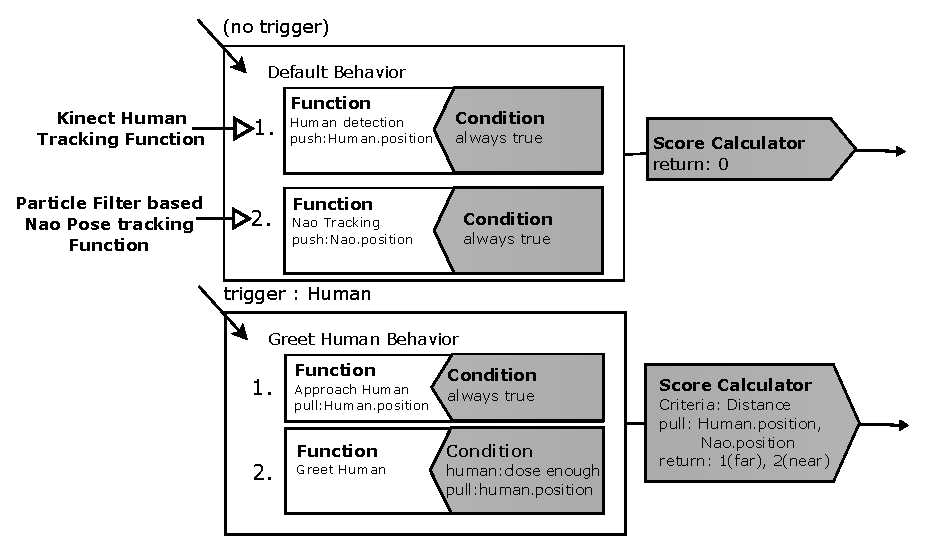
\includegraphics[width=0.8\textwidth]{assets/tdm_example_proposed.eps}
\caption{Greeting a human Example}
\label{fig:program}
\end{figure}	
	The depicted TDM program is just an initial proposal of how the outcome of the work will look like. Once the component library is created, more complex dynamic behavior could be created. The current idea is to design a scenario in which Nao acts as a receptionist and evaluate the interaction using questionnaires and online logging of expression of human. Data analysis will be done using the statistical tools.
\subsection{Research Schedule}
	The research will be carried out in GVLab affiliated to Tokyo University of Agriculture and Technology (TUAT) in Japan under the guidance of Prof.Gentiane Venture. The proposed schedule of the thesis is from \emph{16/02/2015} $\sim$ \emph{18/08/2015}. A more detailed schedule is shown in Figure~\ref{fig:schedule}.
	
\clearpage
\begin{landscape}
\begin{figure}
\centering
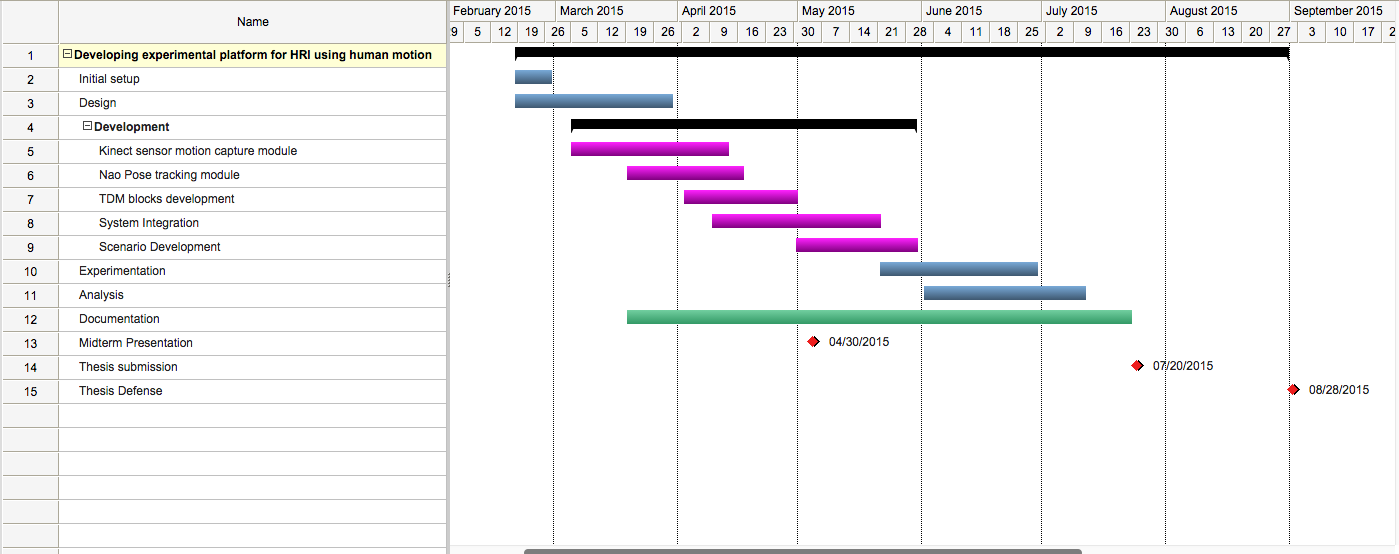
\includegraphics[width=\hsize]{assets/schedule.png}
\caption{Master Thesis tentative schedule}
\label{fig:schedule}
\end{figure}
\end{landscape}
%\section{Experimentation Plan}

\section{Conclusion} % Main chapter title
	Human Robot Interaction is a complex interdisciplinary problem that needs expertise in various fields like human computer interaction, psychology, biomechanics, humanoid robotics etc., Social robots have become very common in the recent days and they find useful applications in entertainment, education, autism treatment and elderly care. 
	
	For an efficient interaction with human, the robot has to understand his motions and also the environment around him. This is only possible when the robot has necessary perception capabilities which seemlessly make the robot understand the human motions. However the onboard sensors most often cannot deliver all the information necessary for an effective interaction. So there is a need to augment exteroceptive sensors to the system and RGB-D sensors prove to be a convincing solution to this purpose. Irrespective of the underlying perception system used, there is also a need for a scalable robot behavior design framework which could take care of automatic information flow between various components in the system and dynamic creation of behaviors based on object permanence in the environment. Combining the perception system and behavior framework will result in a platform wherein interaction based on human motion will be possible. 
	
	This bibliographic study explained the requirements and challenges in each of the problems of motion understanding, robot localization, behavioral design and evaluation techniques. The state of the art research helped to make appropriate choices to tackle each of the problems under study. More specifically in the research plan described in this study, it is proposed to use Kinect V2 sensor as the perception system and use of Kinect SDK for human motion understanding. The robot localization and tracking problem will be tackled by using a parallelized implementation of particle filter tracking algorithm available in Point cloud library. The Target Drives Means(TDM) framework will be used as the dynamic behavior design infrastructure. An example TDM program is also presented that uses the aforementioned experimental platform. The state of the art HRI evaluation techniques like self assesments and behavioral measures will be used to evaluate the interaction. The experimental platform this thesis aims to achieve will encourage diverse experiments focusing on the evaluation of specific interaction metrics.